\documentclass[a4paper,oneside,titlepage]{report}
\usepackage[pdftex]{graphicx}
\usepackage{hyperref}
\usepackage{natbib}
\usepackage{amsmath}
\usepackage{anysize}
\usepackage[a4paper,margin=1in]{geometry}
\usepackage[usenames]{color}
\usepackage{varioref}
\usepackage{verbatim}
\usepackage[latin1]{inputenc}
\usepackage{url}

\bibliographystyle{plainnat}
\bibpunct{(}{)}{;}{a}{,}{,}

\newcommand{\coderef}[2]{\texttt{#1:#2}, page \pageref{code:#1}}
\newcommand{\software}[1]{\texttt{#1}}
\newcommand{\note}[1]{\begin{itemize}
	\item \textcolor{blue}{#1}
\end{itemize}}

\title{Interpolative Playlist Generation}
\author{Jamil George Bashi (92432)\\
\small Supervisor: Nick Collins\\[2cm]
\large BSc Music Informatics\\
\small Informatics / School of Science and Technology}
\date{\Large 2007}

\begin{document}
% This should contain your name, your degree programme and department, 
% your candidate number, the title of the project, the name of your 
% project supervisor and the calendar year of submission.
\begin{titlepage}
\begin{center}
%\thisfancyput(3.25in,-4.5in){%
%  \setlength{\unitlength}{1in}\fancyoval(7,9.5)}

\includegraphics[width=0.5\linewidth]{front/images/us-logo}\\[1cm]

\textsc{\Large Final year project}\\[0.5cm]

\hrulefill \\[0.4cm]
{ \huge \bfseries Similarity Measure for Interpolative Playlist Generation}\\[0.4cm]

\hrulefill \\[1.5cm]
\begin{minipage}{0.4\textwidth}
\begin{flushleft} \large
\emph{Author:}\\
Jamil George \textsc{Bashi} (93432)
\end{flushleft}
\end{minipage}
\begin{minipage}{0.4\textwidth}
\begin{flushright} \large
\emph{Supervisor:} \\
Nick \textsc{Collins}
\end{flushright}
\end{minipage}

%\maketitle
\end{center}
\end{titlepage}

\setcounter{page}{1}
\pagenumbering{roman}
\section*{Abstract}
Blah blah blah
\bigskip


\tableofcontents
\thispagestyle{empty}

\pagenumbering{arabic}
\setcounter{page}{1}

\pagestyle{plain}
\pagenumbering{arabic}
\chapter{Introduction (600/500)}
\begin{comment}
	\item rationale
	\item purpose
	\item issues
	\item context
	\item relevance
	\item structure of dissertation
\end{comment}
In recent years, advances in digital audio compression techniques as well as the ever-increasing popularity of the Internet and on-line music stores have allowed the home computer user to amass a large amount of music with relative ease; the storage and retrieval of music has become simple enough that a purchased album need only be a few clicks away. Despite this, the method of playback has remained unchanged, with most users selecting and playing back an album at a time, with interfaces analogous to selecting and playing back a record, tape or CD. It is possible to create a \emph{playlist}, where the user can add individual songs to a queue, which can be saved and loaded alongside the media library.

While creating playlists allows the user to listen to a variety of music in a session, it is a long and difficult process to find, preview and select a number of songs which will fit the \emph{context of use}, such as listening to music while working, exercising or cleaning. Software such as the system described in this report provide \emph{playlist generation} to the user, aiming to ease the selection of music fitting the context of use and allow the user to listen to music in a new way.

Interpolative playlist generation involves the user specifying a set of \emph{key tracks}, with a specified number of songs between them. The system then `fills the gaps' between these, generating playlists with a smooth musical transition between the keys. Selecting music to play in this manner allows the user to generate playlists by example, rather than having to precisely specify the content with semantic attributes such as year published or genre.

In order to select music for playlist generation, a metric is described which works solely on audio data by using statistical functions to estimate perceptual similarity between tracks. Songs similar to the keys are used to fill the playlist, based on a set of rules of `good' playlist generation.

The system, once developed, would hope to create novel and interesting playlists either equivalent to or better than a user could themselves. The difficulty in this lies in what is known as the automated music transcription problem \citep{Hainsworth2004}; it is very difficult for a human to be able to listen to a recording and re-write the score from which it came and as of such is an unsolved problem in computational music research. Even with a full transcription of a piece, it is impossible for a computer system to accurately measure similarity, due to the lack of understanding of mood or context of a piece. Current similarity metrics aim to overcome this either by inferring similarity through attributes such as artist and genre tags (tracks by the same artist are most likely similar, for example), or by using models of audio perception, and hence are by nature inaccurate. Interpolative playlist generation reduces the reliance on an overly accurate similarity metric by guiding the system through the playlist; in addition, a method for training the system based on an expert user's input of similar tracks is described.
\section{Structure of Dissertation}
This report contains a full description, evaluation and analysis of a music similarity metric and playlist generator developed during my final year of study. I will begin by giving a review of current similar research and software in the area of playlist generation and music similarity measure, and go on to describe and implement a method for interpolative playlist generation. After implementing these techniques, they will be tested on a corpus of tracks from an example music library, and the performance and accuracy of the implemented methods evaluated.

\chapter{Review of Existing Systems}
\section{Outline}
Music Information Retrieval (MIR) is a relatively young topic involving the study of musical content analysis, modelling and archiving to provide semantic search and retrieval of music from large databases. MIR is already in use in a number of commercial projects, such as Shazam!, a service where songs can be identified over a telephone; MusicBrainz adds metadata to stored audio using fingerprinting techniques. 
In order to discover strengths and weaknesses in the area of playlist generation which the system will build upon, four current playlist generation software packages have been trialled by the author and reviewed.
\section{Concepts}
Before discussing the software implementations, it is important to define the terminology used in the area, and the distinction between the main methods of similarity measure and playlist generation. Two areas exist in music similarity metric research; symbolic and sub-symbolic. Symbolic metrics work on the preexisting metadata of the track, such as the artist and album names stored alongside, or using \software{ID3} tags inside, the audio data itself. Generally, statistics are recorded on the user's listening habits such as skipping behaviour \citep{Pampalk2005a}, play counts or user specified ratings, and these are used to determine songs that the user likes and would hence work well in a playlist together. Systems such as these are inherently flawed: if music is labelled incorrectly, has missing metadata, or no recorded statistics, it cannot be used with symbolic similarity metrics. Sub-symbolic systems aim to overcome this by operating directly on the audio data to measure similarity. The system `listens' to the music itself, and uses records characteristics of the audio to either replace or complement the data used in symbolic systems.

When operating on audio data, similarity metrics fall into two groups, again with the distinction of symbolic or sub-symbolic. Symbolic similarity metrics in this sense work on transcribed music, comparing the similarity of melodies on a note-by-note or tonality basis, similar to how a spelling corrector measures similarity between misspelled words and possible corrections. While this can provide great precision, it says nothing about how the music is perceived by the listener, and two songs of differing genre, while they may be similar would most likely be regarded as very dissimilar to a symbolic metric. Sub-symbolic metrics, on the other hand, model a listener's perception of a song, assigning values to attributes used to describe music such as brightness, energy and tempo.
\section{Software}
Most (if not all) current publicly available software for playlist generation use symbolic techniques to infer similarity and generate playlists. Ruffle is a plugin to Muine, a popular Linux audio player, which provides the ability to either generate playlists or extend user-created ones based solely on play counts and the genre tagged in songs. It works well when a large amount of data has been collected and provides an easy-to-use interface to playlist generation. Apple have implemented a similar system in their iTunes software called ``Party Shuffle''. The entire media library is played in random order, biased towards highly-rated or often played songs, and allows the user to remove tracks from the upcoming playlist at will, replacing these with other suggestions. While popular, iTunes and Ruffle offer only a weighted-random approach to playlist generation, with no consideration of continuity of genre or mood.

The Filter is a newly released plugin for Apple's iTunes which amasses play count data from all of its users into a central database. Using such metadata as tempo and genre, along with user's listening habits, it improves on iTunes' Party Shuffle by introducing the concept of continuity. The user is asked to specify a few `seed' tracks, which are then looked up in the on-line database and used to set the mood/genre for the generated playlist.
\section{Literature}
\citet*{Aucouturier2002a} suggest a similarity measure based on a Gaussian mixture model (GMM) of Mel frequency cepstral coefficients (MFCCs). Implemented for playlist generation by \citet{Schnitzer2003}, it works well to measure similarity between tracks returning a number of good results. This technique was later implemented for the CUIDADO project by \citet*{Aucouturier2003}, using an adaptive constraint satisfaction algorithm based on four constraints of no repetition, a desired length, continuity in genre and progression in the theme of the playlist. The benefits of this technique are its high scalability and accuracy, working well with a library of around 200,000 tracks.

\citet{Logan2001} present an alternative similarity metric based on k-means clustering of spectral features, using ``song trajectories'' to create interesting playlists. To test the playlist generation using this technique, a `baseline' playlist was created of the most similar $n$ songs, which was then compared to one using song trajectories. The outcome of this testing showed that it actually performed worse than the baseline playlist, but more promising results were shown when symbolic data was added to guide the metric.

A fully symbolic playlist generation system is described by \citet{Pauws2002}. Personalised Automatic Track Selection (PATS) is a system developed to ease the selection of music for a given context of use, such as listening to soft or lively music. It uses metadata attribute similarity along with a dynamic clustering technique to generate playlists, which were described to have higher coverage of the library, higher precision in selecting similar tracks, and a higher user rating than a baseline playlist of random tracks. This system has a unique method of training, in that users can specify tracks to be dropped from the playlist and using a decision tree, the system trains the weights of the similarity metric. 
\section{Review and Identification of Problem Areas}
Playlist generators based on symbolic analysis such as \software{Ruffle} and \software{The Filter} have two shortcomings: the fact that play counts for each track are their only source of data for statistical analysis, and the reliance on well tagged audio for the similarity metric. \software{The Filter} improves upon this by correlating data between all its users, but still is unable to perform any playlist generation where the songs are completely untagged or `unseen' in the database. Additionally, these techniques rely on the user only listening to artists similar to each other, not accounting for users having wide tastes in music or even simply randomly listening to tracks from the whole library, as the order of tracks played is recorded.

Two systems (Aucouturier and Logan's) have been reviewed detailing systems which are based on sub-symbolic analysis of the audio data in order to overcome the problems with existing symbolic systems. While these have had mixed results, it is a promising area of study and would, depending on the accuracy of the similarity metric developed, provide a more suitable playlist generation without the shortcomings of depending on accurate symbolic data.

In order to comprehensively test the system designed, it will be tested in a method similar to PATS; as well as statistical testing showing the performance of the similarity metric, a small group of users will be interviewed to gain insight into how well the system performs overall and the quality of the playlists generated from the standpoint of the target audience.

% Body of report - this should include a requirement analysis and specification of the problem you have tackled.
%
%%%%%%%%%%%%%%%%%%%%%%%%%%%%%%%%%%%%%%%%%%%%%%%%%%%%%%%%%%%%%%%%%%%%
%                      JUSTIFY ALL MY CHOICES                      %
%%%%%%%%%%%%%%%%%%%%%%%%%%%%%%%%%%%%%%%%%%%%%%%%%%%%%%%%%%%%%%%%%%%%
%
\newcommand{\objective}[1]{
	\subsubsection{#1}
}
\chapter{Specifications and Requirement Analysis (2074/2000)}
\section{Overview}
% set out what my software has to do
In order to investigate music similarity measure and its use in interpolative playlist generation it is important for me to write a proof-of-concept piece of software which is capable of performing these functions, to show that the concepts discussed and my method proposed and designed are solid.

\note{Why specify system behaviour}
I have created a detailed specification of system behaviour in order to focus the development of this system. As stated in \citet{Bourque2004}, ``The Software Requirements Knowledge Area (KA) is concerned with the elicitation, analysis, specification, and validation of software requirements. It is widely acknowledged within the software industry that software engineering projects are critically vulnerable when these activities are performed poorly''. By specifying what is required of the software, and the requirements of the software itself, it becomes easier to design a system based around those goals and hence have a more succinct design and implementation. Additionally, later comparing the final system back to these specifications allows me to both critique the system in terms of how well it met its goals, but also assess the viability of the system (or a future system based on the technique) for development into an end-user application.
\section{System Objectives}
\subsection{Research Requirements}
\note{Why did I set out an objective in the intro?!}
As the system is merely a proof-of-concept version of the similarity measure and playlist generation technique discussed in this paper, it is important that the system lend itself to extensive testing, and be easily extensible and adaptable should I need to change the operation of any component. The following are a set of requirements of the software for research: 
\objective{Provide a method to verify and view results at each step of the processing}
Verification and the ability to view input and output data of the system is important during the development process in order to ensure the correct operation of the code, and to track down any bugs which may arise. Tracking data flow through each step of the system can help to show any areas which may be operating incorrectly or suboptimally.

To achieve this, I will design the system so that it is easy to debug, as well as providing a tool to view any binary files which may be stored. Also, where necessary, I will create program options which will reveal more detailed output about the operation of the system for testing and debugging purposes.
\objective{Provide a simple method to analyse music and create playlists in batch for testing}
% reading compressed files
As I will need to process a large amount of audio files (the user's media library), and generate lots of playlists for testing and debugging, it is important to have an interface to the program which allows for this. I have chosen to use a command-line interface, with the mode of operation and the files to process specified on the command-line, and all output printed to the standard output and error streams. This simplifies the code needed to process options, and allows me to create batch scripts which can automate testing. Also, operating without a GUI eases debugging of the system, which is important for the above requirement.
\objective{Allow components to be added and modified without (severely) affecting the operation of others}
% Encapsulation / Abstraction
Seperating the concerns of similarity measure (audio processing and analysis) and playlist generation (statistical analysis) into seperate programs means that the code itself will be simpler and clearer, which in turn means that it is easier to understand, develop, and test. As I will be modifying the algorithm with which the similarity measure and playlist generation works, it is important that the two do not depend on each other more than necessary. Following the Object-Oriented design philiosophy, and it's ideas of abstraction and encapsulation, I have written the software in \software{C++}, and seperated the program logic into seperate classes, each dealing only with their own data and processing.
\subsection{User Requirements}
In addition to the requirements for me as the developer and researcher, it is important to consider the needs of the hypothetical end-user, who would use a system based upon the technique later discussed. By setting out the requirements for a viable playlist generating application, I can design my system and technique around this. The following are a set of base-line requirements for a feasable playlist generation system.
\objective{Analyse the user's media library in a reasonable time-frame}
Digital signal processing and audio analysis such as required by any audio-based similarity measure requires a great deal of data processing - audio must be read from disk byte-by-byte and calculations performed based on this - if a typical song (uncompressed) is 20MB, this translates to 5,242,880 floating-point additions and a division just to calculate the mean value! As the processing done on each song is immense, it is important to have this processing run as quick as possible, and avoid the need to re-process any one song.

To achieve the kind of speed needed, \software{C++} is a good choice of language as it is a very low-overhead, high speed language. As the amount of calculation required is unavoidable, I will attempt to avoid the need to re-calculate data for a file by storing the analysed data along with the audio files themselves; this means that if files are moved, the analysis data is moved with them.
\objective{Avoid storing too much data}
\label{text:spec:requirement:data}
If too much data for each song is stored it affects the scalability of the application, as for large media libraries the analysis data itself will take up a large amount of disk space. Additionally, the more data stored, the more calculation needed to compute similarity, increasing the time taken to generate playlists exponentially.
\objective{Provide a simpler method of playlist generation than selecting individual tracks}
Playlist interpolation easier to select yadda yadda 
\objective{Base playlist generation solely on analysis of audio data}
relate to problems with other software found in review
\subsection{Extensions}
\objective{Provide a GUI for ease of use}
\objective{Provide a version which can run on portable devices (MP3 players, etc.)}
% The system which I have designed and created is a small demonstration system, tailored for ease and speed of development as development time is limited, verifiability of results to ensure correct operation of the system, and ease of testing outputs to assess the overall performance of the system.
\section{Requirement Analysis}
In addition to analysing what is required of the system, it is important to look at what will be required by the system itself. After looking at the requirements and functionality set out above, I have set out a list of software requirements of the system.
\subsection{Operating System}
Quick note about writing for linux as it's easier? Code kept very portable, relying on libraries helps this.
\subsection{Software Libraries}
Throughout the development of the system, I have made extensive use of software libraries where possible to speed development time and reduce errors. As there are many software libraries available to aid in any individual task, I have evaluated several options and give reasons for each choice.
\subsubsection{Audio Decoding}
Digital audio, when converted to analog for playback or processed in some way is read as a continuous stream of floating-point numbers between 1 and -1, representing the current level of the waveform. When stored on disk, however, there are hundreds of file formats, each with a different set of features and an entirely different algorithm for obtaining the floating-point numbers needed for processing. In a typical user's media library, there can be audio of very different types: MP3 for portable devices, AAC on Apple machines, WMA on Windows, FLAC for lossless compression, WAV for uncompressed audio; it is important that any signal analysis system is able to process at least these types in order to not be unusable. For the purposes of this proof-of-concept code, I began by using \software{libsndfile}[REF], which can read uncompressed audio files (such as WAV and AIFF). While this was suitable for development work, it quickly became evident that if a large number of audio files were to be processed, I would need to be able to decode compressed audio (mainly MP3 and FLAC in my test corpus). Due to this, I used the \software{GStreamer} multimedia framework to decompress, downsample and mix audio to mono (\coderef{SoundFile.cc}{21}) into a temporary WAV file, ready to be read in by libsndfile (\coderef{SoundFile.cc}{29}). While this provides a simple solution to the problem, it is not optimal as it induces the large overhead of spawning another process and writing to a temporary file; again a trade-off with development time and optimality, I could have directly implemented reading from the major formats using their individual libraries, gaining processing speed and reducing overhead.
\subsubsection{Audio Analysis / DSP}
For the audio analysis section of the system, it was possible to use a number of software libraries to implement the signal processing and analysis. \software{Marsays}[REF], \software{MAAATE}[REF] and \software{libaudiofeat}[REF] are three libraries which allow the developer to pass in audio data and receive analysis data. Although this would have avoided the need to directly implement feature extractors (discussed later), it would mean sacrificing both speed in unneeded calculations (\software{libaudiofeat}) and flexibility in the feature extractors (\software{Marsyas} and \software{MAAATE}) which I could use. Also, as these were large and complex libraries, it would have taken me as long to learn how to use the library as it would write the code myself; due to this, I decided to manually implement and test the feature extractors.
The feature extraction process required the computation of a Fourier Transform. As this is a complex mathematical procedure I used the \software{FFTW3} library to perform the computation, as it is a highly optimised library specifically for doing Fourier Transforms.
\subsubsection{User Interface}
As discussed previously, I opted to implement a command-line interface. In order to parse the options specified on the commandline, and provide a unified interface to the user, I used the \software{libpopt} library to parse command-line options. Although this could have been implemented manually, much of the code of libpopt would need to be duplicated and would provide no real benefit.
\begin{comment}
	\begin{itemize}
		\item Give background on libraries used and what they are used for
		\item Give alternatives to some libraries and explain why they wern't used (Marsyas and MAAATE)
		\begin{itemize}
			\item lack of knowledge of libraries - would have taken as long to learn it as to have written it myself
			\item too big to leverage into the proof-of-concept example needed
			\item wouldn't allow as much flexibility in operation of the program
			\item this way is easier to modify in future to add more extractors / build on in any way
			\item why they would have been good
			\begin{itemize}
				\item easier to chop and change between features (not important for my project)
				\item ?
			\end{itemize}
		\end{itemize}
		\item GStreamer (vs. libmad, libogg/vorbis, libflac; directsound)
		\item libsndfile
		\item FFTW3 (vs. hand coded - OMG)
		\item libpopt (vs. hand coded - just lazy)
	\end{itemize}
\end{comment}
\subsection{Hardware \& Storage}
\begin{itemize}
	\item Hardware
	\begin{itemize}
		\item Fast processor
		\item Lots of HDD space for music itself, not much on top of that
	\end{itemize}
	\item Storage
	\begin{itemize}
		\item Seperate files easier to code \& debug
		\item Database slightly less reliable (moved files need to be recalculated) but much faster \& tidier
		\item Data stored on each track needs to be small so as not to take too much disk space
	\end{itemize}
\end{itemize}
% It should also include a description of how you have designed, built and evaluated your system.
% The exact form of this will vary from project to project but it will usually occupy several chapters
% and will often include sections on implementation and testing. Any software projects should included a 
% discussion of the principles which underlie the program which has been written: the significance of its data
% structures, the way that its procedures and modules interact etc.



\chapter{Method, Design, and Implementation (3468/3500)}
%%%%%%%%%%%%%%%%%%%%%%%%%%%%%%%%%%%%%%%%%%%%%%%%%%%%%%%%%%%%%%%%%%
% NEED TO TALK ABOUT THE IMPORTANCE OF SIMILARITY MEASURE TO     %
% THE PERFORMANCE OF PLAYLIST GENERATION, AND HOW INTERPOLATION  %
% ALLOWS THE SIMLIARITY MEASURE TO BE LESS RELIABLE              %
%%%%%%%%%%%%%%%%%%%%%%%%%%%%%%%%%%%%%%%%%%%%%%%%%%%%%%%%%%%%%%%%%%
\section{Overview, Theory \& Principles}
% Talk about how this works (decode audio, extract features, measure similarity, interpolate) as a general overview
The system I have designed provides interpolative playlist generation based on sets of data calculated about each song in the user's media library. The process begins by running the \executable{extractor} program on each of the files in the media library, which begins the process of extracting data about each song known as \emph{features}. These features, calculated from the audio data itself, aim to be an absolute measure of the ``characteristic elements'' \citep{Fingerhut2004} of the sound (or \emph{timbre}), by using statistical functions to gain values based on psychoacoustics. That is to say, ideally, the extracted features become an absolute measure of the timbre of the song, such that two songs with similar features will sound similar. Once these features have been extracted and stored, the \executable{generator} program reads the stored feature vectors into memory and generates a playlist by measuring the distance between the feature vectors, hence giving the \emph{similarity} between songs.

When measuring the similarity between songs, \executable{generator} biases the distance between songs according to a set of \emph{feature weights}, which are a measure of how important each of the features are towards an overall accurate similarity metric. The weights themselves are `trained' by analysing the output of a quiz (\executable{listenertest.rb}), asking the user of the system to pick the two most similar from three clips of songs from the library, a technique suggested by \citet*{Novello2006}. This both allows the system to train itself as to which features are important, but also later assess its own output (with the \executable{evaluate.rb} program) based on how well the similarity metric matches up with the answers given in the quiz.

Interpolative playlist generation involves the user inputting a set of \emph{key songs} and an amount of tracks to add. The system then, using the similarity measure, `fills the gaps' with tracks creating a smooth musical transition in genre between the keys. \citet{Pauws2002} states that ``if it is known that a set of songs is preferred (or fit a given context-of-use), then it is likely that preference can be generalized to other songs based solely on the fact that they are similar''. For example, if asked to interpolate one song between a blues and a hip-hop track it may pick a rhythm-and-blues track, in order to create as smooth a transition as possible. As well as selecting the `best' tracks to create the playlist, the generator also obeys rules of good playlist writing, such as not having songs by the same artist close to each other in the playlist (to add variety to the playlist). Appendix \ref{app:system_diagram} (page \pageref{app:system_diagram}) shows the conceptual layout of the system.
\begin{figure}[ht]
	\caption{Key to mathematical symbols}
	\begin{tabular}{l l}
		$\oplus$		& The exclusive OR operator \\
		$a$				& The vector containing amplitudes for each bin returned from the Fast Fourier Transform (FFT) \\
		$A$				& The vector of feature blocks for song $A$ \\
		$A'$			& The vector of sorted blocks in song $A$ \\
		$f$				& The feature vector for each block \\
		$f_n^{A_{i}}$	& The feature $n$ of song $A$, block $i$ \\
		$F$				& The vector containing frequencies of each bin of $a$ \\
		$g_{i,j}(A,B)$	& The distance between block $i$ of song $A$ and block $j$ of song $B$ \\
		$g_{s,s}$		& The distance between the song feature vectors of song $A$ and song $B$ \\
		$N_B$			& The number of bins returned by the FFT \\
		$N_F$			& The number of features in the vector \\
		$N_G$			& The number of blocks in song $A$ or $B$ (whichever is less) \\
		$N_R$			& The number of results from listener testing \\
		$N_S$			& The number of samples in one window \\
		$s$				& The vector containing signal data for one window \\
		$sgn()$			& Function returning 1 if positive, 0 if negative \\
		$w$				& The feature weights vector \\
		$W_S$			& The weight for the song block \\
		$W_B$			& The overall weight for the song blocks \\
		$v_i(A)$		& Sorting value for block $i$ of song $A$ \\
	\end{tabular}
\end{figure}
\section{Feature Extraction}
% the point of all these is that they each represent part of the sound of a song so that once you've got all the values out you have a measure of what it sounds like to your brain so a song that produces similar values by this measure are similar songs
When analysing an audio file to extract features, the system must first decode the compressed audio. This is performed by calling the external \software{gst-launch} program provided by \software{GStreamer} (\codepageref{SoundFile.cc}{21}) to decode to a temporary file, which is then read in using \software{libsndfile} (\coderef{SoundFile.cc}{45}); once the file has been fully processed, the temporary file is removed (\coderef{SoundFile.cc}{39}).

The audio file is read in 1024-sample (0.02 second) \emph{windows}, which are then passed to \software{FFTW3} (\codepageref{FFT.cc}{44}) to perform the Fourier transform. These two sets of data for each window are then passed to the relevant feature extractors, which return their features for each window (\codepageref{Features.cc}{94}). The features for each window, held by the \executable{FeatureSet} class, are then grouped into 150-window (3.5 second) blocks (\executable{FeatureGroup}s), where their mean, variance, skewness and kurtosis are calculated (\coderef{Features.cc}{29}). The reason for grouping the windows into these blocks is two-fold: first, it provides a two-tiered feature vector to the similarity measure, as all windows are processed into one song-level block at the end of processing (\codepageref{extractor.cc}{119}), which can provide a rough but much less computationally expensive similarity measure; second, it cuts down on the amount of data stored for each track (and hence helps meet the requirement of not storing too much data) while still providing information on the change in features over the track, and allows the standardised moments to be easily calculated.
\begin{figure}[h]
	\centering
	\caption{A processing block from the beginning of \emph{Quick and to the Pointless} by \emph{Queens of the Stone Age}: It begins with ``Yeah yeah yeah yeah!'', the fourth ``yeah'' being overlaid with the entry of the guitar, with three claps towards the end.}
	\subfigure[Waveform (the signal read from the audio file)]{\label{fig:method:block:waveform}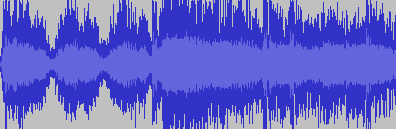
\includegraphics[width=0.5\textwidth]{method/waveform}}
	\subfigure[Spectrogram (a graphic representation of the spectrum returned by \software{FFTW3})]{\label{fig:method:block:spectrogram}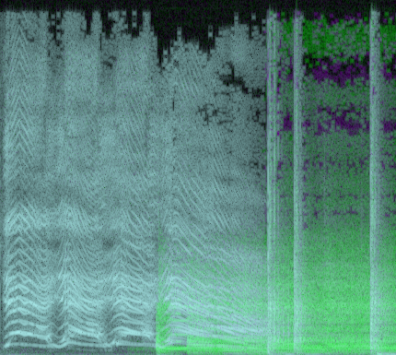
\includegraphics[width=0.5\textwidth]{method/spectrogram}}
	\label{fig:method:block}
\end{figure}
\subsection{Standardised Moments}
For each feature extracted the mean, variance, skewness and kurtosis over each three second block are calculated. It is these four values that are then used in the similarity measure, as it is unnecessary to store the output of each feature extractor for each window (and the amount of data would exceed what was set out in the specification, page \pageref{text:spec:requirement:data}). These values show how each feature for each window changes over the course of a block: variance describes how much the values change; skewness, how asymmetrical the data set is; and kurtosis, the `peakedness' or `flatness' of the data set \citep{Siegrist2007}.
\subsection{Signal Descriptors}
Signal descriptors are values which are calculated from the values of the audio data itself and tend to be values based on the periodicity or short-time amplitude of the signal. They are aggregate functions working directly on values stored in the audio files, and as of such are much less computationally expensive than the spectral descriptors, which require the output of an F. As is shown by figure \ref{fig:method:block:waveform}, it is easy to see the changes in amplitude, shape and periodicity as a whole from the waveform, but discerning polyphonic events is difficult (the fourth ``yeah!'' is almost completely obscured by the entry of the guitar).
\subsubsection{Zero Crossing Rate}
\begin{equation}
\mathit{Zero Crossing Rate} = \frac{1}{N} \sum_{i=0}^{N-2} sgn(s_i) \oplus sgn(s_{i+1})
\label{eq:zero_crossing_rate}
\end{equation}

The zero crossing rate is the number of times the signal passes from positive to negative or vice versa; it can be used as primitive pitch detection algorithm, and has been used successfully in the classification of percussive sounds \citep{Gouyon2000} and speech recognition[REF], due to the fact that it tends to be higher and unstable during the attack period of a sound \citep{Schwarz2004}.
\subsubsection{First Order Autocorrelation}
\begin{displaymath}
\mathit{FirstOrderAutocorrelation} = \frac{1}{N_S} \sum_{i=0}^{N_S-2} s_i \cdot s_{i+1}
\label{eq:first_order_autocorrelation}
\end{displaymath}

Autocorrelation is a measure of how well the signal matches a time-shifted version of itself, and hence shows the `noisiness' of the signal. \citep{Wikipedia2007}. As with zero crossing rate, this is useful to find attacks as well as being a measure of the harshness of the timbre of the sound.
\subsubsection{Energy}
\begin{displaymath}
\mathit{Energy} = \frac{1}{N_S} \sum_{i=0}^{N_S-1} (s_i)^2
\label{eq:energy}
\end{displaymath}

Energy gives a linear measure of the total amplitude in each window, giving an approximation of the perceived `loudness' of the sound. This will be useful for determining the level of change in energy per block, and hence be a measure of the distinctiveness of beats.
\subsection{Spectral Descriptors}
Spectral descriptors use Fourier series (the output of a discrete Fourier transform); rather than working in the dimensions of amplitude and time, they output values from the dimensions of frequency and amplitude. Figure \ref{fig:method:block}, \vpageref{fig:method:block}, shows the data analysed for one block of audio for both the spectral and signal descriptors. Spectral descriptors, working in the frequency domain, aim to represent features of the timbre of the sound, with the higher statistical moments looking at the change in timbre over blocks.
\subsubsection{Linear Regression}
\begin{equation}
\beta = \frac{n \sum (xy) - \sum x \sum y}{n \sum x^2 - \sum x^2}
\label{eq:linear_regression}
\end{equation}

Linear regression finds the line of best fit through a set of data. This statistical approximation has been used to find the gradient ($\beta$) of the spectrum, which is a measure of the ratio of high-frequency to low-frequency component of the sound and hence the timbre. With this feature the variance will most likely be a valuable similarity measure, as it will show the smoothness of timbre - long sustained notes will have low variation in linear regression, fast or noisy music will have a large variance.
\subsubsection{Centroid}
\begin{equation}
\mathit{SpectralCentroid} = \frac{\displaystyle \sum_{i=0}^{N-1} a_i f_i}{\displaystyle \sum_{i=0}^{N-1} a_i} 
\label{eq:spectral_centroid}
\end{equation}

The spectral centroid is analogous to the centre of gravity of a set of data if it were imagined to be a 2D shape \citep{Park2004}; it represents the average frequency weighted by amplitude, and hence where most of the energy of the signal lies. Psychoacoustically it is a measure of the perceived `brightness' of the sound, providing a better estimation of a `bright' sound than pitch \citep{Schubert2004}, and tending to rise for more intense sounds. This feature will represent the timbre of each block as a whole, and provide information on the change in timbre through the song.
\subsubsection{Smoothness}
\begin{equation}
\mathit{SpectralSmoothness} = \sum_{i=0}^{N-1} 20 \log a_i - \frac{20\log a_{i-1} + 20\log a_{i} + 20\log a_{i+1}}{3}
\label{eq:spectral_smoothness}
\end{equation}

Smoothness, also known as flatness, can be used to obtain a measure of the spectral envelope (the change in spectrum over time) of a sound \citep{Klapuri2003}. It is a measure of how spread out the signal is across the spectrum --- white noise, which has power at all frequencies, would have a smoothness of around 1; a sine wave, on the other hand, would have a smoothness of 0, as it is a single spike in the spectrum \citep{Peeters2004}. Using this, the smoothness will give a good measure of the noisiness and harmonicity of the signal.
\subsubsection{Spread}
\begin{equation}
\mathit{SpectralSpread} = \sqrt{\frac{\sum_{i=0}^{N-1} a_i (f_i - \mathit{SpectralCentroid})^2}{\sum_{i=0}^{N-1} a_i}}
\label{eq:spectral_spread}
\end{equation}

Spectral spread describes the variance of the signal about its spectral centroid \citep{Peeters2004}, and hence the perceptual `width' of the timbre. Orchestral or `full-sounding' tracks will have a large spread, whereas a monophonic or solo performance will produce smaller values.
\subsubsection{Dissymmetry}
\begin{displaymath}
\mathit{SpectralDissymmetry} = \sqrt{\frac{\sum_{i=1}^{N_B} a_i (F_i - \mathit{SpectralCentroid})^3}{\sum_{i=1}^{N_B} a_i}}
\label{eq:spectral_dissymmetry}
\end{displaymath}

Dissymmetry (or skewness) is a measure of how skewed the spectrum is about the spectral centroid, and hence the tilt towards high or low frequencies. Along with smoothness and spread, this is another extractor gaining values about the shape of the spectrum; in this case, a measure based on the harmonicity of the sound near the spectral centroid.
\subsection{Commentary}
For the system designed, eight feature extractors have been implemented, each aiming to be an absolute measure of a part of the timbre of a track, in order to later measure the similarity. The feature extractors used were chosen through evaluation of the development time alotted, processing time required and performance of the system. While it would have been possible to implement more, such as the MFCC used by \citet{Schnitzer2003} and \citet{Aucouturier2002a} or the range available with \software{Marsyas}, increasing the number of feature extractors would not necessarily increase accuracy, and would require more development and processing time.
\section{Similarity Measure}
\label{text:method:similarity_measure}
The similarity measure, performed by \executable{generator} (in \codepageref{Song.cc}{162} and \codepageref{Features.cc}{46}), works on the features stored by \executable{extractor}. When \executable{generator} is run, it begins by loading the analysis files / feature vectors for each of the songs in the media library (\codepageref{SongSet.cc}{21}). These are then normalised into the range 0--1, in order to avoid any feature having bias over others due to its values being larger (the difference between two centroids could be several thousand; when added to the distance between two linear regressions which are $-1$ to 1, the centroid would have much more effect on the similarity than the regression). When \executable{generator} is run with the \texttt{-s} command-line option, it performs a similarity measure against a specified track and every other track in the database, returning the top $n$ matches, so that the similarity measure can be tested alone from the playlist generation.

To compute the similarity between two songs, \executable{generator} computes the difference between two feature blocks using the following equation:
\begin{equation}
g_{i,j}(A,B) = \sum_{n=0}^{N_F-1} w_n | f_n^{A_i} - f_n^{B_j} |
\label{eq:feature_block_distance}
\end{equation}
\begin{center}
	\small \textit{(where $i$ and $j$ are $s$ for the song blocks of song $A$ and $B$)}
\end{center}

That is, the total of the absolute value of each feature subtracted from the corresponding feature in the second block, multiplied by the corresponding weight.

As the feature blocks extracted from the audio are sequential three-second clips, the similarity measure is very dependant on both the tempo of the music and the order of the blocks when compared to another song. If the beats happen to fall at the same rate as the blocks are extracted (roughly 69 or 138bpm, the energy measure will be inflated and not match the `true' timbre. Likewise, the structure of the song will affect the features extracted as the timbre of the verse will be substantially different from the chorus (for example), therefore putting more emphasis on the order of comparisons. This has been overcome in two ways: first, the overall song feature block is the average timbre of the entire track, and hence is not affected by the structure of the song; second, four different methods of comparing the feature blocks have been implemented and evaluated, each with their own advantages for the overall similarity metric.

\label{text:method:comparison_methods}
\subsubsection{Ordered Comparison}
\begin{equation}
s_o(A,B) = W_S g_{s,s}(A,B) + W_B \frac{\sum_{i=0}^{N_G-1} g_{i,i}(A,B)}{N_G}
\label{eq:song_distance_ordered}
\end{equation}

The first algorithm implemented was the simple ordered comparison: block 1 in song 1 is compared to block 1 in song 2, block 2 to 2 and so on. This similarity measure will be strongly affected by the structure of the two tracks: if the same song is compared to one with three seconds of silence at the beginning, it will return a similarity much lower than it should. However, by being so reliant on structure, it will rank similar-structured songs as more similar, therefore possibly working better for already-similar tracks such as a set of tracks from the same album.
\subsubsection{Ordered Area Comparison}
\begin{equation}
s_a(A,B) = W_S g_{s,s}(A,B) + W_B \frac{\sum_{i=1}^{N_G-1} g_{i,i-1}(A,B) + \sum_{j=0}^{N_G-1} g_{j,j}(A,B) + \sum_{k=0}^{N_G-2} g_{k,k+1}(A,B)}{3N_G-2}
\label{eq:song_distance_ordered_area}
\end{equation}

The area comparison hopes to improve on the ordered comparison (\ref{eq:song_distance_ordered}) by additionally comparing the previous and next block from song B with song A, thereby comparing each block from song A with a nine second area in song B. Comparing songs in this way means that the comparison still takes structure into account, but is less reliant on the structural changes happening at the same time in two tracks for a low similarity measure. Additionally, by comparing three groups at once, the problems with the timings of the song aligning with the block boundaries are alleviated.
\subsubsection{Exhaustive Comparison}
\begin{equation}
s_e(A,B) = W_S g_{s,s}(A,B) + W_B \frac{\sum_{i=0}^{N_G-1}\sum_{j=0}^{N_G-1} g_{i,j}(A,B)}{{N_G}^2}
\label{eq:song_distance_exhaustive}
\end{equation}

Exhaustive comparison aims to get a `complete' comparison of the two tracks, by comparing each block from song A to each in song B, and hence is not affected by the structure of the song in any way. This is also the only comparison which takes the whole of both songs into account, regardless of length. This means that it will provide much better results than the other comparisons in the case of songs $A$ and $B$ having greatly different length, but will be the slowest of all comparisons to compute.
\subsubsection{Sorted Block Comparison}
In the sorted block comparison, the feature blocks from both songs are both sorted according to the sum of their normalised features:
\begin{equation}
v_i(A) = \sum_{n=0}^{N_F-1} f_n^{A_i}
\label{eq:feature_block_sorting_value}
\end{equation}

The songs are then compared in the same way as the ordered comparison:
\begin{equation}
s_s(A,B) = W_S g_{s,s}(A',B') + W_B \frac{\sum_{i=0}^{N_G-1} g_{i,i}(A',B')}{N_G}
\label{eq:song_distance_sorted}
\end{equation}

This approach is similar to the exhaustive comparison in that it is unaffected by structure, but provides a rough (and hence much less expensive) comparison between already similar blocks in the two songs (as they have been sorted by their total), meaning it will be focusing on much smaller differences between features, and hence work best for finding very similar tracks even if the structure is disparate.
\subsection{Commentary}
As the way to compare blocks that will result in the best overall accuracy is unknown, four different algorithms have been implemented and later evaluated. Although some algorithms may work better than others in specialisation, it is beyond the scope of this project to explore using combinations of these for increased accuracy. Attempting to implement this would require a testing mechanism with the kind of accuracy required to evaluate fine-tuning of the similarity measure, though it would be considered as a future extension.
\section{Playlist Generation}
\executable{generator}, when run in playlist generation mode, is supplied with a list of key songs and a number of tracks to add between. Once the feature vectors have been loaded and normalised (see page \ref{text:method:similarity_measure}), the playlist generator creates a new empty playlist of the correct length, with the key tracks in position (stored as an array of \executable{PlaylistEntry}s, \codepageref{Playlist.cc}{60}). The \executable{PlaylistEntry}s hold arrays of tracks, sorted in descending order of their similarity to the `ideal' track for that position in the playlist, created by interpolating between the song feature block of the two neighbouring key tracks (\coderef{Playlist.cc}{28}). At this stage, the playlist holds the closest matches to the ideal tracks, ie.\ the `best' playlist. To avoid repetition of artist and hence improve the variation \citep{Pauws2002}, the playlist generator then groups together tracks by the same artist between the same two key songs (\coderef{Playlist.cc}{112}), and scores them based on how similar they are to their ideal track for that position in the playlist (\coderef{Playlist.cc}{33}). The track which is best for that position in the playlist is kept, and the others are resorted with the artist in question removed. This process is repeated until no tracks remain with the same artist, when the playlist is outputted as a list of files relative to the media library folder (the M3U format).

The similarity measure used when sorting the tracks based on their similarity to the ideal track works solely on the song features, in order to cut down on the processing required to generate a playlist. If the playlist generator were to sort using the similarity to a set of interpolated feature blocks, each song in the media library would have to be compared multiple times to the `ideal' feature blocks, and it would be very computationally expensive. When calculating the score of each track (when removing artists), the feature blocks are taken into account to obtain a better similarity metric, and an weight added to the song features ($W_S$) and feature blocks ($W_B$) to bias the scores so they are not too dissimilar between the two similarity metrics.

Interpolative playlist generation in this manner reduces the reliance on a highly accurate similarity measure, as the metric is `guided' between tracks. Also, as repeated artists are excluded from the playlist, often the most similar track is skipped in favour of one with a different artist. It is only important for the similarity measure to return tracks with a roughly similar mood and timbre, so as not not `stick out' in a playlist --- the variety created by such a method is more important than a highly accurate measure of distance between songs.
\section{Weight Optimisation}
\label{text:method:weight_optimisation}
As it is not completely understood how we perceive sound and music, feature extractors only work as a basic model to return statistics based on the timbre of the sound; it is therefore best to use a number of these models and let empirical evidence from testing `teach' the system which of these best represent measures which can determine the similarity of audio. It is important for the system to have a vector of weights, which bias the comparison of songs towards certain features, in order to gain a more accurate similarity measure. The weight vectors represent a set of ratios of how important each feature is to the overall similarity measure; some features will be more useful to the similarity measure than others, and biasing towards these will improve the performance of the system.

The weights are trained through analysis of a user's answers to a \emph{music quiz} (\codefilepageref{listenertest.rb}), which asks the user to pick which two of three tracks played are the most similar. The results are then analysed, increasing the relevant weights according to features which were similiar in the two tracks given, using the algorithm shown in \ref{eq:weight_optimisation_old}.
\begin{equation}
w_i = \sum_{n=0}^{N_R-1} 1 - |f_i^{K_n^s} - f_i^{S_n^s}|
\label{eq:weight_optimisation_old}
\end{equation}
\begin{center}
	\small \emph{(where $f_i^{K_n^s}$ is feature $i$ of the song block of key song $n$, $f_i^{S_n^s}$ being the given similar track)}
\end{center}

Training in this manner allows the system to learn which features are important based on the user's estimate of similar tracks. Due to the length of time required to gather results (playing three extracts takes 30 seconds each, so it is a slow and labourious process, though training need only be done once) and hence the small amount of training data possible, the system considers tracks on the same album to be similar (especially true in the case of a compilation album) and uses these to further train itself, though giving less emphasis to these results as they were not specified by the user.

In addition to using tracks from the same album a source of similar track data, it would be possible as a future development to also query existing symbolic systems such as \software{Last.fm} or \software{Ruffle} for similar tracks and use these for training, providing the similar tracks returned by those systems are present in the user's media library.

The results from the music quiz can be used both in training and in testing, to determine how well the system learns and how accurate the similarity measure is. When provided with the results of the quiz, the system adjusts the weights aiming to return results more similar to the ones provided; the `perfect' system would, after training, give results identical to the training set while still having the ability to generalise to other music not used in the training. Using this, it is possible to automatically evaluate the efficacy of the system based on how close its results are to the user's responses, before and after testing.
\section{Critique of Design and Implementation}
The overall design of the system meets the specification well; the intensive audio processing happens once and is stored, playlist generation then being a much less intensive (and hence faster) process. Data is summarised during processing, reducing the data storage (~20KB per song) and subsequent processing time. To aid debugging, a data viewer has been provided, which produces warnings about invalid numbers. In the similarity measure where it is unknown which algorithm will work best, four algorithms have been implemented and will later be tested. A method for training and testing the system based on a user's `expert' input has been detailed, aiming to train the weights and hence denote more or less important features to the similarity metric.

Due to the object-oriented approach to the structure of the code, it is easy to extend and adapt. Once such improvement which could be made would be to pre-calculate distances between every track in the library, greatly reducing the computation required to generate playlists, possibly allowing the playlist generation to run on a portable device such as an MP3 player.

\newcommand{\graph}[2]{
\begin{figure}[!hp]
	\caption{#2}
	\includegraphics[width=\textwidth]{testing/graphs/#1}
	\label{graph:#1}
\end{figure}}
\chapter{Testing (3282/1000)}
\label{text:testing}
Testing the functioning, performance and accuracy of the system allows for evaluation as to how well the system meets its specification and purpose. Additionally, testing will help identify strengths, weaknesses, and areas for improvement of the system. Three approaches have been taken to the testing: functional, which will test that the system works as designed and meets specifications; automated testing, giving a measure of the algorithms used and their affect on results; and user testing, gaining feedback on the performance of the system as an accurate similarity metric and playlist generator.
\section{Functional Testing}
\label{text:testing:functional}
To show correct operation of the system and give examples of generated playlists, excerpts of the output of the program are given along with some example queries and their output.
\subsection{\executable{extractor}}
For this test, the feature extractor was run on three tracks from \emph{Kasabian}'s album, \emph{Empire}.\\
Command:
\begin{verbatim}
./extractor ../test/Kasabian/Empire/Empire-04-Me\ Plus\ One.mp3 \
    ../test/Kasabian/Empire/Empire-06-Apnoea.mp3 \
    ../test/Kasabian/Empire/Empire-08-Stuntman.mp3
\end{verbatim}
Output:
\begin{verbatim}
../test/Kasabian/Empire/Empire-04-Me Plus One.mp3: decode, analyse, done (83 blocks)
../test/Kasabian/Empire/Empire-06-Apnoea.mp3: decode, analyse, done (60 blocks)
../test/Kasabian/Empire/Empire-08-Stuntman.mp3: decode, analyse, done (181 blocks)
\end{verbatim}

The three tracks were processed, and the features written out to files on disk, 12KB, 8KB and 24KB in size respectively.
\subsection{\executable{viewer}}
To show the operation of \executable{viewer}, it was run on one of the feature vectors outputted by \executable{extractor} above, to show the feature blocks (output summarised).\\
Command:\\
\verb"./viewer -b ../test/Kasabian/Empire/Empire-04-Me\ Plus\ One.mp3.vec"\\
Output:
\begin{alltt}
"Block","Mean of Zero Crossing Rate","Variance of Zero Crossing Rate","Skewness of Zero\ldots
1,0.0482357,0.00052548,0.251996,2.37784,0.0329947,0.000534037,1.97615,7.77386,0.00112283,\ldots
2,0.047806,0.000511404,0.0219624,1.97833,0.0325186,0.000534909,1.70473,6.22687,0.00110232,\ldots
3,0.0476497,0.000567088,0.465436,2.74142,0.0310403,0.000429462,1.70945,6.72855,0.00104859,\ldots
4,0.0786003,0.00558258,2.66379,10.0214,0.0388259,0.000730849,1.59315,6.35009,0.00128985,\ldots
5,0.0915951,0.00356234,1.46339,4.70598,0.0555432,0.00101183,1.40148,5.28068,0.00183747,\ldots
\end{alltt}


As can be seen from the inspection of the first feature, the track begins with a repeated guitar riff, followed by the later entry of the vocals which can be seen by the rising values of the mean of zero crossing rate. This simple test shows that the feature extractor works correctly, and that the features change with events in the track.
\subsection{\executable{listenertest.rb}}
The following is an example run of the listener test:\\
Command:
\begin{verbatim}
./listenertest.rb
\end{verbatim}
Output:
\begin{verbatim}
Loaded 1456 songs

-------------------------------------------------------------
Listen to these three extracts, and choose which two are the most similar:
Song A, Song B or Song C? (enter ? for help)
?
[A,B,C][A,B,C] - Answer
L[A,B,C] - Listen to clip again
I[A,B,C] - Get track info
S - Skip
Q - Quit
Song A, Song B or Song C? (enter ? for help)
S

-------------------------------------------------------------
Listen to these three extracts, and choose which two are the most similar:
Song A, Song B or Song C? (enter ? for help)
LC
Song A, Song B or Song C? (enter ? for help)
BC

-------------------------------------------------------------
Listen to these three extracts, and choose which two are the most similar:
Song A, Song B or Song C? (enter ? for help)
Q
Thanks!
\end{verbatim}

The results from the test are then stored in \texttt{results.txt}.
\subsection{\executable{learner}}
\label{text:testing:functional:learner}
After all songs were processed and the listener test was performed to gain around 100 results, the learner was run to calculate a set of weights:\\
Command:
\begin{verbatim}
./learner --dir=../test
\end{verbatim}
Output:
\begin{verbatim}
1413 songs loaded
{ 0.613092, 0.205134, 0.533735, 0.110462}, 
{ 0.306893, 0.132636, 0.453016, 0.0505156}, 
{ 0.321113, 0.183988, 0.485224, 0.0169958}, 
{ 0.459398, 0.206291, 0.48236, 0.260304}, 
{ 0.279731, 0.121066, 0.449003, 0.0465693}, 
{ 0.677096, 1, 0.786617, 0.545458}, 
{ 0.997773, 0.680246, 0.306549, 0.0242729}, 
{ 0.718418, 0.303971, 0.29711, 0}
\end{verbatim}

As the weights are normalised in the range 0--1, it provides a human-readable estimation of the importance of each feature for the similarity measure. Table \ref{table:weights} is a labelled description of the weights:
\begin{table}[!hbp]
\caption{Weights outputted by \executable{learner}. The best and worst results in each column and row are coloured green and red respectively.}
\label{table:weights}
\centering
\begin{tabular}{|l|l|l|l|l|l|}
\cline{2-6}
\multicolumn{1}{l|}{} & Mean & Variance & Skewness & Kurtosis & \textbf{Mean} \\ 
\hline
Zero Crossing Rate & 0.6131 & 0.2051 & 0.5337 & 0.1105 & 0.3656 \\ 
\hline
First Order Autocorrelation & 0.3069 & 0.1326 & 0.4530 & 0.0505 & 0.2358 \\ 
\hline
Linear Regression & 0.3211 & 0.1840 & 0.4852 & 0.0170 & 0.2518 \\ 
\hline
Spectral Centroid & 0.4594 & 0.2063 & 0.4824 & 0.2603 & 0.3521 \\ 
\hline
Energy & 0.2797 & 0.1211 & 0.4490 & 0.0466 & \bad{0.2241} \\ 
\hline
Spectral Smoothness & 0.6771 & \good{1} & 0.7866 & 0.5455 & \good{0.7523} \\ 
\hline
Spectral Spread & 0.9978 & 0.6802 & 0.3065 & 0.0243 & 0.5022 \\ 
\hline
Spectral Dissymmetry & 0.7184 & 0.3040 & 0.2971 & \bad{0} & 0.3299 \\ 
\hline
\textbf{Mean} & \good{0.5467} & 0.3542 & 0.4742 & \bad{0.1318} & \multicolumn{1}{l}{} \\ 
\cline{1-5}
\end{tabular}
\end{table}


As can be seen from the weights returned, the mean of each feature proved the most valuable, along with spectral smoothness as by far the most important extractor. The energy performed the worst of all extractors perhaps due to it's variability; the gain of the recording (how loud it is recorded/stored) will directly affect this extractor---it would perhaps work better if the tracks were normalised before or during processing.

The kurtosis of each feature extractor faired much worse than expected. This is perhaps due to the nature of the processing: features are collected in three-second blocks and it would be unusual to see a rise and fall to create a peak in features in one block.

The weights returned by \executable{learner} were pasted into the code of \executable{generator} and recompiled, to be used in subsequent testing.
\pagebreak
\subsection{\executable{generator}}
\subsubsection{Similarity Measure}
For the first test, the playlist generator was run to provide the 50 most similar tracks to the given song, \emph{Quick and to the Pointless} by \emph{Queens of the Stone Age}. NB: there was only one \emph{Queens of the Stone Age} track in the media library, hence no others appearing in the results. The distance for each track appears in brackets after the file name.\\
Command:
\begin{verbatim}
./generator --verbose --similar=50 --comparison=sorted --dir=../test \
../test/Queens\ of\ the\ Stone\ Age/Rated\ R/Rated\ R-07-Quick\ and\ to\ the\ Pointless.mp3.vec
\end{verbatim}
Output: \small \emph{(Line numbers have been added for ease of reference)}
\begin{listing}{1}
../test/nofx/The Greatest Songs Ever Written (By Us)/The Greatest Songs Ever Written (By Us)-24-It's My Job to Keep Punkrock Elite.ogg (0.297521)
../test/Rancid/Rancid/Rancid-17-Meteor of War.mp3 (0.305863)
../test/The Distillers/Sing Sing Death House/Sing Sing Death House-05-Sing Sing Death House.mp3 (0.310962)
../test/Various Artists/BYO Split Series, Volume V/BYO Split Series, Volume V-03-Alkaline Trio-Dead and Broken.mp3 (0.314302)
../test/Rancid/Rancid/Rancid-06-Poison.mp3 (0.318846)
../test/Alkaline Trio/Remains/Remains-13-Dead and Broken.mp3 (0.320534)
../test/The Distillers/Sing Sing Death House/Sing Sing Death House-10-Desperate.mp3 (0.322074)
../test/nofx/The Greatest Songs Ever Written (By Us)/The Greatest Songs Ever Written (By Us)-25-Franco Un-American.ogg (0.325217)
../test/Junior Senior/Hey Hey My My Yo Yo/Hey Hey My My Yo Yo-08-Ur a Girl.mp3 (0.326607)
../test/Various Artists/Mob Mentality/Mob Mentality-02-The Business-In the Streets of London.mp3 (0.327603)
../test/Rancid/Rancid/Rancid-07-Loki.mp3 (0.331062)
../test/Rancid/Rancid/Rancid-13-Not to Regret.mp3 (0.33118)
../test/Various Artists/Punk-O-Rama, Volume 10/Punk-O-Rama, Volume 10-27-Roger Miret and the Disasters-Riot, Riot, Riot.ogg (0.332419)
../test/Various Artists/Mob Mentality/Mob Mentality-08-The Business-Borstal Boys.mp3 (0.336915)
../test/Alkaline Trio/Goddamnit/Goddamnit-02-Cop.mp3 (0.341494)
../test/Rancid/Rancid/Rancid-09-Rejected.mp3 (0.34587)
../test/Various Artists/Punk-O-Rama, Volume 10/Punk-O-Rama, Volume 10-20-Rancid-White Knuckle Ride.ogg (0.346863)
../test/Rancid/Rancid/Rancid-14-Radio Havana.mp3 (0.347537)
../test/nofx/The Greatest Songs Ever Written (By Us)/The Greatest Songs Ever Written (By Us)-06-Bleeding Heart Disease.ogg (0.352109)
../test/The Distillers/Coral Fang/Coral Fang-05-Coral Fang.mp3 (0.354196)
../test/Alkaline Trio/Crimson (bonus disc)/Crimson (bonus disc)-01-Time to Waste (demo).mp3 (0.355211)
../test/Rancid/and Out Come the Wolves/and Out Come the Wolves-12-She's Automatic.mp3 (0.355757)
../test/Alkaline Trio/Good Mourning/Good Mourning-03-One Hundred Stories.mp3 (0.355769)
../test/Alkaline Trio/Crimson (bonus disc)/Crimson (bonus disc)-05-Dethbed (demo).mp3 (0.356513)
../test/Alkaline Trio/Maybe I'll Catch Fire/Maybe I'll Catch Fire-08-She Took Him to the Lake.mp3 (0.358377)
../test/Various Artists/BYO Split Series, Volume V/BYO Split Series, Volume V-08-One Man Army-The Hemophiliac.mp3 (0.360446)
../test/Alkaline Trio/Good Mourning/Good Mourning-07-Fatally Yours.mp3 (0.359591)
../test/Alkaline Trio/Good Mourning/Good Mourning-14-Old School Reasons.mp3 (0.360203)
../test/Four Tet/DJ-Kicks Four Tet/DJ-Kicks Four Tet-09-Animal Collective-Baby Day.mp3 (0.357063)
../test/Various Artists/BYO Split Series, Volume III/BYO Split Series, Volume III-07-NOFX-I'm the One.mp3 (0.360754)
../test/Alkaline Trio/Good Mourning/Good Mourning-06-Emma.mp3 (0.361064)
../test/System of a Down/Mezmerize/Mezmerize-03-Revenga.mp3 (0.361441)
../test/nofx/The Greatest Songs Ever Written (By Us)/The Greatest Songs Ever Written (By Us)-05-Murder the Government.ogg (0.36334)
../test/Alkaline Trio/Remains/Remains-16-Wait for the Blackout.mp3 (0.364695)
../test/Alkaline Trio/Crimson (bonus disc)/Crimson (bonus disc)-06-Settle for Satin (demo).mp3 (0.364749)
../test/Rancid/Rancid/Rancid-08-Blackhawk Down.mp3 (0.365072)
../test/Basement Jaxx/Rooty/Rooty-01-Romeo.flac (0.365695)
../test/Alkaline Trio/Alkaline Trio/Alkaline Trio-09-For Your Lungs Only.mp3 (0.365721)
../test/Rancid/Rancid/Rancid-05-Another Night.mp3 (0.366004)
../test/Rancid/Rancid/Rancid-18-Dead Bodies.mp3 (0.366937)
../test/System of a Down/Mezmerize/Mezmerize-02-B.Y.O.B..mp3 (0.367975)
../test/Various Artists/Punk-O-Rama, Volume 10/Punk-O-Rama, Volume 10-14-Converge-Black Cloud.ogg (0.368253)
../test/Goldfinger/The Best of Goldfinger/The Best of Goldfinger-03-Miles Away.mp3 (0.368692)
../test/Rancid/Rancid/Rancid-21-Reconciliation.mp3 (0.370021)
../test/Saves the Day/Can't Slow Down/Can't Slow Down-10-Hot Time in Delaware.mp3 (0.372484)
../test/The Distillers/Sing Sing Death House/Sing Sing Death House-04-The Young Crazed Peeling.mp3 (0.373146)
../test/Rancid/Rancid/Rancid-11-Antennas.mp3 (0.373572)
../test/Rancid/Rancid/Rancid-10-Corruption.mp3 (0.373799)
../test/Rancid/Rancid/Rancid-10-Injury.mp3 (0.374139)
../test/Alkaline Trio/Remains/Remains-09-Old School Reasons.mp3 (0.37425)
\end{listing}


This example query shows a high accuracy in similarity measure---track one is very similar in all aspects, and the tracks following slowly reduce in similarity. The first \emph{outlier} is \emph{Junior Senior}, track 9, which does not appear very similar at all. Continuing on from that, the tracks only become dissimilar enough to not sit well in a playlist from track 29 onwards, though still continuing in order of similarity, suggesting a good long-range accuracy of the similarity measure. 
\subsubsection{Playlist Generation}
To test the playlist generation, two playlists were generated to highlight difficulties in creating `good' playlists with the technique described: a short playlist between two tracks disparate in genre (as it is difficult to create a smooth progression with only a small amount of tracks), and a long playlist between two similar songs (as finding tracks by \emph{different artists} which can create a smooth transition is difficult).

First, the short playlist, between a fast-paced aggressive track by \emph{System of a Down}, and a slow, calm and atmospheric track by \emph{Four Tet}.\\
Command:
\begin{verbatim}
./generator --comparison=sorted --interpolate=3 --dir=../test
    ../test/System\ of\ a\ Down/Mezmerize/Mezmerize-04-Cigaro.mp3.vec
    ../test/Four\ Tet/Pause/Pause-08-No\ More\ Mosquitoes.mp3.vec
\end{verbatim}
Output: \small \emph{(Line numbers have been added for ease of reference)}
\begin{listing}{1}
../test/System of a Down/Mezmerize/Mezmerize-04-Cigaro.mp3
../test/Saves the Day/Sound the Alarm/Sound the Alarm-01-Head for the Hills.mp3
../test/RJD2/Since We Last Spoke/Since We Last Spoke-02-Exotic Talk.mp3
../test/Basement Jaxx/Rooty/Rooty-02-Breakaway.flac
../test/Four Tet/Pause/Pause-08-No More Mosquitoes.mp3
\end{listing}


Second, the long playlist, between two tracks by \emph{Saves the Day}, both melodic, up-beat songs with vocals.\\
Command:
\begin{verbatim}
./generator --comparison=sorted --interpolate=15 --dir=../test ../test/Saves\ the\ Day/In\ Reverie/In\ Reverie-05-In\ Reverie.mp3.vec ../test/Saves\ the\ Day/In\ Reverie/In\ Reverie-01-Anywhere\ With\ You.mp3.vec
\end{verbatim}
Output: \small \emph{(Line numbers have been added for ease of reference)}
\begin{listing}{1}
../test/Saves the Day/In Reverie/In Reverie-05-In Reverie.mp3
../test/Every Time I Die/Hot Damn!/Hot Damn!-06-Floater.mp3
../test/The Prodigy/The Dirtchamber Sessions, Volume One/The Dirtchamber Sessions, Volume One-02-Various Artists-Section 2: Bug Powder Dust  Pump Me Up  How High  Poison  Been Caught Stealing  I Get Wrecked.flac
../test/Alkaline Trio/Alkaline Trio/Alkaline Trio-08-Cooking Wine.mp3
../test/Gescom/Minidisc/Minidisc-82-Hemiplegia 2.mp3
../test/Collide/Some Kind of Strange/07 Mutation.flac
../test/Mindless Self Indulgence/Frankenstein Girls Will Seem Strangely Sexy/Frankenstein Girls Will Seem Strangely Sexy-12-Holy Shit.mp3
../test/Four Tet/Dialogue/Dialogue-05-Misnomer.mp3
../test/Silverstein/Discovering the Waterfront/Discovering the Waterfront-09-Already Dead.mp3
../test/Transplants/Haunted Cities/Haunted Cities-11-I Want It All.mp3
../test/Goldfinger/The Best of Goldfinger/The Best of Goldfinger-04-Superman.mp3
../test/Squarepusher/Big Loada/Big Loada-10-Significant Others.mp3
../test/88 Fingers Louie/Behind Bars/Behind Bars-05-Smart Enough to Run.mp3
../test/The Sainte Catherines/Dancing for Decadence/Dancing for Decadence-06-Emo-Ti-Cons: Punk Rock Experts.mp3
../test/Rancid/Let's Go/Let's Go-13-Ghetto Box.mp3
../test/The Avalanches/Since I Left You/Since I Left You-02-Stay Another Season.mp3
../test/Saves the Day/In Reverie/In Reverie-01-Anywhere With You.mp3
\end{listing}


It can be seen that in both playlists, \executable{generator} found difficulty in generating a `good' playlist while still adhering to the no-repeated-artists rule. In the short playlist, the middle track by \emph{RJD2}, works well as a half-way point between the two tracks posessing a similar beat and tempo to the \emph{Four Tet} track, while still having similar instrumentation to the \emph{System of a Down} track. The \emph{Saves the Day} and \emph{Basement Jaxx} are not as similar as would have been hoped and do not fit well in the progression due to their differing genres, though they do posess similar rhythm and instrumentation to the two neighbouring tracks.

In the second playlist, where \executable{generator} had to interpolate 15 tracks between two very similar songs the same pattern as the previous was shown, where the middle track (\emph{Already Dead} by \emph{Silverstein}) was a good half-way point, similar to both key tracks. The other tracks, however, showed an interesting progression, as the genre of the tracks seemed to work towards and away from the center while not being similar to the two key tracks, suggesting some improvement needed in the selection of tracks to drop in the case of repeated artists.
\pagebreak
\section{Automated Testing}
As discussed previously (in Method, page \pageref{text:method:weight_optimisation}), it is possible to use the output from the listener test to rate the system's accuracy before and after training. For each of the results, \executable{evaluate.rb} generates a playlist with each of the four comparison methods. The average position of the similar and not-similar tracks are then taken, along with their standard deviation and the difference between placement of the similar and not-similar track. Low values for the average placement of similar tracks and standard deviation, as well as high values for the difference between similar and not-similar would indicate an accurate system.
\subsection{Results}
Figure \ref{graph:metric-comparison} shows a comparison of the four track comparison methods detailed on page \pageref{text:method:comparison_methods}, before any training (all weights set to 1). While the two algorithms which take structure into account (Ordered and Ordered Area) provided better similar and non-similar placement difference and hence better distinction between tracks, Sorted and Exhaustive had a lower standard deviation, suggesting a more reliable metric. It is clear from these results that the sorted comparison performed the best overall, having a higher average placement of the similar tracks, a relatively high difference between similar and not-similar placement, and a standard deviation much less than that of the ordered area comparison.
\graph{metric-comparison}{Comparison of Similarity Metrics}

To test the efficiency of the training of the system, \executable{evaluate.rb} was run before and after training, to show the affect of training. After an initial test, it was shown that training the system actually provided \emph{worse} accuracy.  To investigate this further, I modified the source code of \executable{learner} to either only train on the albums in the user's media library or on the answers from the listener test, and re-ran the test (figure \ref{graph:training-method-comparison}). As there is more data available for the album training than the test answer training, it can be seen that the more data used in training, the worse the accuracy of the similarity metric, as if the system were training \emph{away} from the data set. On re-evaluating the algorithm used to train the data (formula \ref{eq:weight_optimisation_old}, page \pageref{eq:weight_optimisation_old}), I dropped the subtraction from one, and reran the test. 
\graph{training-method-comparison}{Comparison of Training Methods}

Previously, the algorithm worked by subtracting the distance between features from one, such that two similar features would increase the weight more than two disparate features, which logically seems sound. Figure \ref{graph:training-algorithm-comparison} shows the similar track placement with an untrained system, a trained system, and a system trained with the new algorithm (formula \ref{eq:weight_optimisation_new}).
\begin{equation}
w_i = \sum_{n=0}^{N_T-1} |f_i^{K_n^s} - f_i^{S_n^s}|
\label{eq:weight_optimisation_new}
\end{equation}

\graph{training-algorithm-comparison}{Comparison of Training Algorithms}

The results from the new algorithm proved much better than both an untrained system and one trained with the old algorithm: a reduced mean and standard deviation of placement of similar track, and a much larger difference in similar and not-similar placement. Training the system in the previous manner may have served to smooth the differences between features across the data set, as large differences would end up having a smaller weight and hence be reduced to small differences, and vice-versa. Training in this way does the opposite; large distances between individual features are made larger, and hence tracks would need to be very similar in that feature for it to have a large affect on the overall distance. This new algorithm was used in all subsequent testing, as it has overall better performance.

Table \ref{table:testing_data} provides a summary of data from all tests.
\begin{table}[hp]
	\caption{Testing Data}
	\label{table:testing_data}
	\centering
\footnotesize \begin{tabular}{|l|l|l|l|l|l|l|}
\cline{3-6}
\multicolumn{1}{c}{} &  & \multicolumn{2}{c|}{\textbf{Similar}} & \multicolumn{2}{c|}{\textbf{Not Similar}} & \multicolumn{1}{l}{} \\ 
\hline
\multicolumn{1}{|c|}{\textbf{Training}} & \multicolumn{1}{c|}{\textbf{Metric}} & \multicolumn{1}{c|}{\textbf{Mean}} & \multicolumn{1}{c|}{\textbf{StDev}} & \multicolumn{1}{c|}{\textbf{Mean}} & \multicolumn{1}{c|}{\textbf{StDev}} & \multicolumn{1}{c|}{\textbf{Difference}} \\ 
\hline
\multicolumn{1}{|c|}{\textbf{Untrained}} & Ordered & 469.23 & 354.65 & 807.08 & 420.82 & 337.85 \\ 
\cline{2-7}
\multicolumn{1}{|c|}{} & Ordered Area & 484.39 & 370.1 & \good{827.74} & 428.44 & 343.35 \\ 
\cline{2-7}
\multicolumn{1}{|c|}{} & Sorted & 463.81 & \good{338.19} & 805.23 & 423.69 & 341.42 \\ 
\cline{2-7}
\multicolumn{1}{|c|}{} & Exhaustive & 474.35 & 353.99 & 803.4 & 423.26 & 329.05 \\ 
\hline
\multicolumn{1}{|c|}{\textbf{Both}} & Ordered & 493.97 & 363.67 & 799.74 & 426.5 & 305.77 \\ 
\cline{2-7}
\multicolumn{1}{|c|}{\textbf{Albums}} & Ordered Area & \bad{507.47} & 379.27 & 822.61 & \bad{434.64} & 315.15 \\ 
\cline{2-7}
\multicolumn{1}{|c|}{\textbf{and}} & Sorted & 481.26 & 344.64 & 802.24 & 425.42 & 320.98 \\ 
\cline{2-7}
\multicolumn{1}{|c|}{\textbf{Answers}} & Exhaustive & 499.44 & 364.79 & 796.08 & 428.32 & 296.65 \\ 
\hline
\multicolumn{1}{|c|}{\textbf{Albums}} & Ordered & 493.97 & 363.67 & 799.76 & 426.51 & 305.79 \\ 
\cline{2-7}
\multicolumn{1}{|c|}{} & Ordered Area & \bad{507.47} & 379.27 & 822.61 & \bad{434.64} & 315.15 \\ 
\cline{2-7}
\multicolumn{1}{|c|}{} & Sorted & 481.19 & 344.7 & 802.24 & 425.42 & 321.05 \\ 
\cline{2-7}
\multicolumn{1}{|c|}{} & Exhaustive & 499.44 & 364.79 & 796.06 & 428.31 & \bad{296.63} \\ 
\hline
\multicolumn{1}{|c|}{\textbf{Answers}} & Ordered & 488.85 & 358.98 & 798.69 & 426.93 & 309.84 \\ 
\cline{2-7}
\multicolumn{1}{|c|}{} & Ordered Area & 500.52 & 373.69 & 821.61 & 434.23 & 321.1 \\ 
\cline{2-7}
\multicolumn{1}{|c|}{} & Sorted & 473.39 & 344.12 & 809.07 & 424.57 & 335.67 \\ 
\cline{2-7}
\multicolumn{1}{|c|}{} & Exhaustive & 495.37 & 360.73 & \bad{794.37} & 429.72 & 299 \\ 
\hline
\multicolumn{1}{|c|}{\textbf{New}} & Ordered & 440.6
 & 349.36
 & 811.08
 & 406.04
 & 370.48
 \\ 
\cline{2-7}
\multicolumn{1}{|c|}{\textbf{Algorithm}} & Ordered Area & 445.74
 & \bad{445.74}
 & 825.15
 & 410.98
 & 379.4
 \\ 
\cline{2-7}
\multicolumn{1}{|c|}{} & Sorted & \good{438.15}
 & 438.15
 & 806.5
 & 410.97
 & \good{410.97}
 \\ 
\cline{2-7}
\multicolumn{1}{|c|}{} & Exhaustive & 445.02
 & 445.02
 & 819.97
 & \good{398.63}
 & 398.63
 \\ 
\hline
\end{tabular}
\end{table}

\pagebreak
\section{User Testing}
\label{text:testing:user}
In order to gain valuable user feedback on the performance of the system with regards to similarity measure, three users with prior musical knowledge were asked to comment on playlists generated and a list of similar tracks. Also, to gain insight into the user's listening habits, the users were asked to comment on how they generally listened to music. The results of these interviews are summarised below.
\subsection{Similarity Measure}
The three users were shown the results of a query of the 10 most similar tracks to one of their choosing, and allowed to play and skip between tracks at will. They were then asked to make a few comments on the similarity of each track to the first.
\subsubsection{User A}
User A chose to evaluate the similarity measure on \emph{Roll On} by \emph{Sneaker Pimps}, a down-tempo track with female vocals, a deep bass sound and a punctuated breakbeat rhythm; figure \ref{fig:testing:user:similarity:a}. User A began by saying that the tempo of the first three tracks were greatly increased from the key song chosen. The first four results were overall very similar, especially in instrumentation and rhythm. The first deviation in genre was noted at track five, where there was a ``change of pace and style''. Although the structure and instrumentation were different, the track was still heard to be reasonably similar. User A said that track seven onwards seemed to be almost entirely different in style; it was much slower yet still having similar vocals, which may have caused the similarity measure to rate this track in the top 10 most similar.
\begin{figure}[!hb]
	\caption{Results of a query for the 10 most similar tracks to \emph{Roll On} by \emph{Sneaker Pimps}}
	\label{fig:testing:user:similarity:a}
	\begin{listing}{1}
../test/Sneaker Pimps/Becoming X/02 Tesko Suicide.flac
../test/Fugees/Greatest Hits/Greatest Hits-10-Ready or Not (Salaam's Ready for the Show remix).MP3
../test/The Avalanches/Since I Left You/Since I Left You-06-Flight Tonight.mp3
../test/Sneaker Pimps/Becoming X/05 Spin Spin Sugar.flac
../test/Various Artists/Unsound/Unsound-13-Bad Religion-Los Angeles Is Burning.flac
../test/Rancid/Let's Go/Let's Go-04-Salvation.mp3
../test/Sneaker Pimps/Becoming X/10 Walking Zero.flac
../test/Rancid/Let's Go/Let's Go-05-Tenderloin.mp3
../test/Rancid/Let's Go/Let's Go-17-Dope Sick Girl.mp3
\end{listing}
\end{figure}


It is obvious from the results that while the system was able to find a number of similar tracks, they quickly diminished in similarity, when there are other similar tracks on the same album (\emph{Becoming X}) which were not listed. User A picked up immediately on the changes in tempo for reasons why the tracks were not similar; as the system does not have any feature which is affected greatly by the tempo of the track, adding this may increase similar track selection accuracy.
\subsubsection{User B}
User B chose to evaluate \emph{Colours} by \emph{Hot Chip} (figure \ref{fig:testing:user:similarity:b}), another down-tempo track, this time more electronic with a solid four-to-the-floor beat. As with User A, the immediate observation was that the tempo of the first three tracks was increased, yet the timbre was similar. Track two, while being of a completely different genre, had a very similar timbre, enough that it would be considered perceptually similar.
\begin{figure}[p]
	\caption{Results of a query for the 10 most similar tracks to \emph{Colours} by \emph{Hot Chip}}
	\label{fig:testing:user:similarity:b}
	\begin{listing}{1}
Peaches/The Teaches of Peaches/The Teaches of Peaches-04-Set It Off.mp3
Four Tet/Rounds/Rounds-05-Spirit Fingers.mp3
Serafin/No Push Collide/No Push Collide-09-Sage Waits.ogg
Four Tet/DJ-Kicks Four Tet/DJ-Kicks Four Tet-10-Madvillain-Figaro (101 remix).mp3
Peaches/Impeach My Bush/Impeach My Bush-05-Downtown.mp3
The Postal Service/Give Up/Give Up-04-Nothing Better.ogg
Various Artists/Tijuana Sessions, Volume 3/Tijuana Sessions, Volume 3-02-Fussible-Tijuana Makes Me Happy.mp3
Hot Chip/The Warning/The Warning-02-And I Was a Boy From School.ogg
Bloc Party/A Weekend in the City/A Weekend in the City-05-Uniform.mp3
Saves the Day/Stay What You Are/Stay What You Are-06-Freakish (1).mp3
\end{listing}
\end{figure}


Track four was noted as being an outlier; apart from a similar song structure and perhaps a similar rhythm, it was very dissimilar. Track six was noted as being relatively similar, perhaps moreso than ones previously in the playlist. 7--10 however were said to be quite disparate from the others, though having a similar vocal style.

The similarity metric overall seemed to perform worse than for the track selected by user A. User B suggested that tracks two, three and five were the most similar and should have appeared higher in the ranking, with track one perhaps being in place of track five. To investigate further, \executable{generator} was rerun showing the scores assigned to each track (using the \texttt{-v} flag). The scores returned for the ten tracks were in the range 0.434--0.489, showing that the tracks all occupied a small area in the feature space, possibly accounting for the confusion of ordering of results.
\subsubsection{User C}
User C evaluated \emph{Like Eating Glass (Ladytron Zapatista Remix)} by \emph{Bloc Party} (figure \ref{fig:testing:user:similarity:c}), a repetitive electro remix with vocal samples of the original. User C gave the overall impression that the tracks returned were very similar, especially in tempo, though each differing in one aspect. Track one, while being synthy and repetitive, lacked vocals yet was similar in mood and genre. Track two was more upbeat, yet had very similar rhythm and genre. The first outlier was track four, which was faster, of a completely different genre of mood, and had very dissimilar vocals. The similar sounding percussion and structure however may have accounted for this.
\begin{figure}[p]
	\caption{Results of a query for the 10 most similar tracks to \emph{Like Eating Glass (Ladytron Zapatista Remix)} by \emph{Bloc Party}}
	\label{fig:testing:user:similarity:c}
	\begin{listing}{1}
RJD2/The Third Hand/The Third Hand-13-Paper Bubble.mp3
Transplants/Haunted Cities/Haunted Cities-05-Doomsday.mp3
Whitey/The Light at the End of the Tunnel is a Train/The Light at the End of the Tunnel is a Train-03-Y.U.H.2.B.M.2.mp3
Transplants/Haunted Cities/Haunted Cities-01-Not Today (feat. Sen Dog).mp3
Peaches/The Teaches of Peaches (bonus disc)/The Teaches of Peaches (bonus disc)-04-Felix Partz (remake) (feat. Gonzales).mp3
Aphex Twin/I Care Because You Do/I Care Because You Do-04-Icct Hedral (edit).flac
Various Artists/Unsound/Unsound-07-Matchbook Romance-Surrender.flac
Killswitch Engage/The End of Heartache/The End of Heartache-10-And Embers Rise.ogg
Four Tet/DJ-Kicks Four Tet/DJ-Kicks Four Tet-15-Quickspace Supersport-Superspace.mp3
Peaches/The Teaches of Peaches/The Teaches of Peaches-11-Felix Partz.mp3
\end{listing}
\end{figure}

\subsection{Playlist Generation}
In the next test, the three users were allowed to select three tracks to make a playlist; hence having two interpolation regions. They were then asked to comment on how well the playlist `flowed', ie.\ its continuity.
\subsubsection{User A}
User A chose a playlist with the tracks \emph{X Dummy} by \emph{Trash Palace}, \emph{Leave Them All Behind} by \emph{Whitey} and \emph{Kalamazoo} by \emph{Primus}. Figure \ref{fig:testing:user:playlist:a} shows the results of this query.

User A chose to comment on the second half of the playlist, the interpolation between \emph{Whitey} and \emph{Primus}. It was however noted that two tracks by \emph{Alkaline Trio} appeared in the first half of the playlist, suggesting a bug in how the artist's name is extracted. User A found that while each track was similar in it's own right with no tracks `sticking out' in the playlist, the tracks failed to flow, frequently changing in genre. This did however produce an interesting result in the choice of \emph{The Cinematic Orchestra} for the track preceding the \emph{Primus} key; it was similar both in tempo, rhythm and instrumentation and flowed well into the next track, though proved unexpected as the tracks were from completely differing genres.
\begin{figure}[ht]
	\caption{Playlist generated for User A}
	\label{fig:testing:user:playlist:a}
	\begin{listing}{1}
../test/Trash Palace/Positions/Positions-12-X Dummy.mp3
../test/The Rapture/Pieces of the People We Love/Pieces of the People We Love-09-The Sound.ogg
../test/Various Artists/BYO Split Series, Volume V/BYO Split Series, Volume V-01-Alkaline Trio-Fine Without You.mp3
../test/Alkaline Trio/Alkaline Trio/Alkaline Trio-02-This Is Getting Over You.mp3
../test/Sneaker Pimps/Becoming X/02 Tesko Suicide.flac
../test/Collide/Some Kind of Strange/02 Euphoria.flac
../test/Saves the Day/Saves the Day/Saves the Day-09-The Last Lie I Told.mp3
../test/Transplants/Haunted Cities/Haunted Cities-10-Pay Any Price.mp3
../test/Whitey/The Light at the End of the Tunnel is a Train/The Light at the End of the Tunnel is a Train-02-Leave Them All Behind.mp3
../test/The Avalanches/Since I Left You/Since I Left You-15-Summer Crane.mp3
../test/Collide/Some Kind of Strange/09 Shimmer.flac
../test/Four Tet/Pause/Pause-10-You Could Ruin My Day.mp3
../test/Peaches/The Teaches of Peaches/The Teaches of Peaches-08-Lovertits.mp3
../test/Bloc Party/Silent Alarm Remixed/Silent Alarm Remixed-06-She's Hearing Voices (Erol Alkan's Calling Your dub).flac
../test/Jackson and His Computer Band/Smash/03 Arpeggio.flac
../test/The Cinematic Orchestra/Every Day/Every Day-05-Man With The Movie Camera.mp3
../test/Primus/Brown Album/Brown Album-13-Kalamazoo.mp3
\end{listing}
\end{figure}

\subsubsection{User B}
User B chose \emph{99 Red Balloons} by \emph{Goldfinger}, \emph{Frontier Psychiatrist} by \emph{The Avalanches} and \emph{Lying Is the Most Fun a Girl Can Have Without Taking Her Clothes Off} by \emph{Panic at the Disco} for their playlist, figure \ref{fig:testing:user:playlist:b}. Commenting on the first half of the playlist, user B said that overall the playlist worked well, having a very smooth transition of music towards and away from \emph{The Avalanches}, and having a generally good flow of mood and genre. One problem noted was a very apparent `jump' in genre from track four to five; to investigate this the 50 most similar tracks to track four (\emph{Bad Religion}) were listed. Track five (\emph{Sneaker Pimps}) appeared as the 13th most similar track, with all previous being by artists appearing elsewhere in the playlist. This would mean the reason for the jump in genre was created in the repeated artist exclusion process, as tracks elsewhere were deemed better fitting, forcing this entry in the playlist to choose a track of low similarity.
\begin{figure}[p]
	\caption{Playlist generated for User B}
	\label{fig:testing:user:playlist:b}
	\begin{listing}{1}
Goldfinger/The Best of Goldfinger/The Best of Goldfinger-10-99 Red Balloons.mp3
Rancid/Rancid/Rancid-07-Outta My Mind.mp3
Alkaline Trio/Crimson/Crimson-03-Burn.mp3
Various Artists/Unsound/Unsound-13-Bad Religion-Los Angeles Is Burning.flac
Sneaker Pimps/Becoming X/08 Roll On.flac
Fugees/Greatest Hits/Greatest Hits-10-Ready or Not (Salaam's Ready for the Show remix).MP3
Silverstein/Discovering the Waterfront/Discovering the Waterfront-11-Call It Karma.mp3
Saves the Day/I'm Sorry I'm Leaving/I'm Sorry I'm Leaving-05-I Melt With You.mp3
The Avalanches/Since I Left You/Since I Left You-13-Frontier Psychiatrist.mp3
Boards of Canada/Geogaddi/Geogaddi-02-Music Is Math.flac
RJD2/Since We Last Spoke/Since We Last Spoke-14-Holy Toledo.mp3
Saves the Day/In Reverie/In Reverie-04-Rise.mp3
Various Artists/The Connected Series #2/The Connected Series #2-03-Venetian Snares-How to Steal and Store an Ice Sculpted Bear.mp3
Sneaker Pimps/Becoming X/02 Tesko Suicide.flac
Alkaline Trio/From Here to Infirmary/From Here to Infirmary-12-Crawl.mp3
Peaches/Impeach My Bush/Impeach My Bush-12-Do Ya.mp3
Panic! At the Disco/A Fever You Can't Sweat Out/A Fever You Can't Sweat Out-07-Lying Is the Most Fun a Girl Can Have Without Taking Her Clothes Off.mp3
\end{listing}
\end{figure}

\subsubsection{User C}
User C analysed the first half of a playlist generated with \emph{Gangsters and Thugs} by \emph{The Transplants}, \emph{Superman} by \emph{Goldfiger} and \emph{Ebolarama} by \emph{Every Time I Die} (figure \ref{fig:testing:user:playlist:c}). Similar to the `jump' noted by user B, track two seemed relatively distant from the first to user C. Continuing from this track, the playlist was evaluated to work very well creating a playlist with a smooth transition in genre, though having some tracks of considerably slower tempo (such as track four).
\begin{figure}[!t]
	\caption{Playlist generated for User C}
	\label{fig:testing:user:playlist:c}
	\begin{listing}{1}
Transplants/Haunted Cities/Haunted Cities-03-Gangsters and Thugs.mp3
Collide/Some Kind of Strange/08 Tempted.flac
The Avalanches/Since I Left You/Since I Left You-17-Live at Dominoes.mp3
Whitey/The Light at the End of the Tunnel is a Train/The Light at the End of the Tunnel is a Train-07-HaHaHa.mp3
Basement Jaxx/Rooty/Rooty-01-Romeo.flac
Various Artists/Punk-O-Rama, Volume 10/Punk-O-Rama, Volume 10-08-This Is Me Smiling-Mixin' Up Adjectives.ogg
Rancid/and Out Come the Wolves/and Out Come the Wolves-05-Olympia WA..mp3
Alkaline Trio/Alkaline Trio/Alkaline Trio-05-My Friend Peter.mp3
Goldfinger/The Best of Goldfinger/The Best of Goldfinger-04-Superman.mp3
Various Artists/BYO Split Series, Volume V/BYO Split Series, Volume V-11-One Man Army-I.F.H.A. (One Love).mp3
Alkaline Trio/Good Mourning/Good Mourning-14-Old School Reasons.mp3
The Prodigy/The Dirtchamber Sessions, Volume One/The Dirtchamber Sessions, Volume One-05-Various Artists-Section 5: New York Punk to Funk I'm Sick.flac
Rancid/Let's Go/Let's Go-13-Ghetto Box.mp3
Saves the Day/In Reverie/In Reverie-01-Anywhere With You.mp3
The Sainte Catherines/Dancing for Decadence/Dancing for Decadence-01-Burn Guelph Burn.mp3
Silverstein/Discovering the Waterfront/Discovering the Waterfront-01-Your Sword vs. My Dagger.mp3
Every Time I Die/Hot Damn!/Hot Damn!-08-Ebolarama.mp3
\end{listing}
\end{figure}

\subsection{Blind trialling}
In order to evaluate the overall performance and accuracy of the system, a double-blind test was conducted where the user had to correctly identify a set of three playlists, one created randomly, one by the system, and one by the author. A short overview of the project and the aim of the system was given, in order to give context to the test being performed. The users were allowed as much time as necessary and could freely play back and skip through the three playlists before giving an answer. A short script was written to play back playlists in a random order and the author was not present during testing, in order to eliminate any possible bias in testing.
\subsubsection{User A}
User A correctly identified the three playlists, though having trouble differentiating the manually created and generated ones. The random playlist was quickly identified as the tracks were of very different genres, though user A found the other two playlists to be of very coherent genre throughout. After a number of replays of the manually created and generated playlists, user A came to their decision based on the mood of the tracks; the manual playlist had a more homogeneous and progressive change of mood throughout, whereas the generated one changed mood abruptly towards the end of the playlist.
\subsubsection{User B}
User B also correctly identified all three playlists. The random playlist was identified as it was said to lack coherence: although the tracks sounded similar to user B, there was no flow between the tracks, which seemed to jump between disparate genres with each track. The manually created playlist was identified as there was little progression seen in the playlist, with tracks being similar in groups of two or three songs. User B identified the computer generated playlist with ease, as it was said to have a very smooth transition between songs, with the first and last three songs having very similar opening sections and tempi.
\subsubsection{User C}
\label{text:testing:user:blind:c}
After a great deal of scrutiny user C successfully identified all three playlists, though having trouble distinguishing the three, as the manual and random playlist both appeared quite randomly selected in nature, suggesting the importance of mood in a `good' playlist was overstated. Both the manual and random playlists were said to have abrupt changes in mood and genre, requiring user C to relisten a number of times before the descision was made on the manually created playlist as it seemed to have a progression in tempo towards the final track. The generated playlist was easily identified there were sections in neighbouring tracks that were very similar (generally the intro and chorus), and possessed a very smooth transition in genre.
\section{Critique of Testing Method}
%Work above 90\% will demonstrate understanding of the problems and limitations of evidence and arguments and the means by which they can be overcome
The testing methods used, while designed to be as objective as possible, have a number of shortcomings which could be overcome to produce more accurate and informative results. The automated statistical testing used the training data set to test the functionality of the system; while this proves a useful metric for testing the accuracy of the system, it fails to test the generalisation of the system to music other than that in the test set. To provide an objective test of the generalisation of the system, a larger set of results from \executable{listenertest.rb} would be gathered, which could be split into a test and training set.

The listening test itself could be improved, as currently no feedback is gained from the user about \emph{how} similar the two tracks chosen are. This additional data would both provide a more accurate training algorithm based on the relative similarity of tracks, and a more accurate testing metric comparing the expected and actual placement of tracks in the similarity ranking.

The two subjective tests of similarity measure and playlist generation, while useful to gain feedback on flaws in the model of perceptual similarity measure and playlist generation, provide a rough qualitative measure of the performance of the system, easily swayed by the user's appreciation of a genre of music or musical education. A set of playlists generated by expert users could be used to train the system based on empirical evidence; again if this were split into a training and test set, a quantative measure of the quality of a playlist could be developed.

\chapter{Analysis (1500)}
\begin{itemize}
	\item Subject the findings to scrutiny as to what they might mean
	\item Discussion and analysis of the theories, ideas, issues and challenges noted earlier in the writing. Do you have both intended and unintended outcomes?
	\item A `making sense' of the findings by considering their implications for the questions raised
	\item A critique of the research method (data collection tools?) used and their validity and reliability
\end{itemize}
\section{Accuracy}
\note{how well the system performs as a similarity measure and subsequent playlist generator}
\section{Efficacy}
\note{how well the system as a whole meets the specifications, either reiterate them or refer back}
\section{Weaknesses}
\begin{itemize}
	\item NaN problems
	\item requirement of pre-processing tracks, speed of processing
	\item similarity measure could have higher accuracy
	\item similarity measure doesn't consider mood or genre
	\item explain why the system doesn't have provisions for exploring the library (variance)
\end{itemize}
\begin{itemize}
	\item Album effect, \citet*{Kim2006}
	\item evaluating similarity measures \citet*{Aucouturier2004}
	\item Automatic Music Transcription, transcription problem, symbolic similarity measure from subsymbolic data \citet*{Aucouturier2004}
	\item Structure \citet*{Bruderer2006}
	\item Refinement, training and optimisation, \citet*{Bruderer2006}
	\item Local search, constraint satisfaction \citet*{Vossen2005}
\end{itemize}

\chapter{Summary and Conclusions (500)}
% this should include an assessment of the success of the finished product. Have you achieved your objectives (Terms of Reference)? If not, why not? It should also contain suggestions for future extensions, or alternative methodologies that, with hindsight, might have led to an improvement of the system.
\begin{itemize}
	\item Implications for policy and practice
	\item Recommendations for action
\end{itemize}
\section{Critique: Successes in terms of objectives}
\subsection{Why mine's better than any before! Ha HA!}
\section{Alternative Methodologies}
\section{Future Work and Extensions}


\appendix
\cleardoublepage
\addcontentsline{toc}{chapter}{Bibliography}
\nocite{*}
\bibliography{appendicies/report}


\end{document}

